 
   %judul bisa diketik ulang
  \setstretch{1}%\small
  \begin{center}
      \textbf{\large \Title}\\
      \bigskip 
  \end{center}
  
  
  
  %Nama authors
   \begin{center}
     \bf \Author$^1$, Ade Romadhony$^2$
  \end{center}
  
  
  %Afiliasi dan email
   \begin{center}
      $^{1,2}$Fakultas Informatika, Universitas Telkom, Bandung\\
      $^1$nurcahyo@student.telkomuniversity.ac.id, $^2$aderomadhony@telkomuniversity.ac.id
  \end{center}
  
   
 %%% Abstrak Indonesia %%%%%%%%%%  
   
{\bf \parindent0pt \noindent\rule{\textwidth}{1pt}
Abstrak

Dalam pemrosesan bahasa alami, combinatory categorial grammar (CCG) merupakan salah satu
formalisme tata bahasa yang dapat digunakan untuk membangun sebuah \textit{parser} yang umumnya
dikenal sebagai CCG \textit{parser}.
CCG \textit{parser} dapat digunakan untuk berbagai macam keperluan dalam pemrosesan bahasa alami.
Sebagai contoh, CCG \textit{parser} dapat digunakan untuk memperoleh informasi
(\textit{information extraction}) dari suatu kalimat yang kemudian membentuk sebuah \textit{query}.
Agar dapat membangun CCG \textit{parser} ataupun \textit{tools} lainnya, ketersediaan
\textit{dataset} CCG yang memuat CCG \textit{lexicon} sangat diperlukan. Saat Tugas Akhir ini
ditulis, \textit{dataset} CCG untuk bahasa Indonesia belum tersedia. Demikian itu, CCGtown dibangun
sebagai \textit{annotation tool} yang dapat digunakan untuk membangun \textit{dataset} CCG.
CCGtown merupakan \textit{open source graphical annotation tool} berbasis web yang dirancang
dengan fokus mempercepat serta mempermudah proses penganotasian.
Dengan fitur \textit{generate} CCG \textit{derivation} serta \textit{auto-assign} CCG
\textit{category} kegiatan repetitif dalam melakukan anotasi akhirnya berkurang.
Dengan antarmuka (UI/UX) yang cukup baik menjadikan CCGtown alat anotasi yang mudah digunakan
(\textit{user friendly}) oleh berbagai kalangan pengguna.
% Dokumen ini merupakan panduan penulisan jurnal Tugas Akhir (TA) di lingkungan Fakultas Informatika Universitas Telkom. Meskipun demikian, dimungkinan/dipersilahkan untuk pembimbing TA menggunakan struktur penulisan yang tidak sama persis dengan yang ada di dokumen ini. Panjang abstrak tidak lebih dari 200 kata dan diketik dalam ukuran huruf 10 pts. TA sebagai salah satu sarana latihan penulisan akademik dan memperjelas tulisan, abstrak dibagi menjadi empat paragraf atau sub-bagian. Setiap sub bagian bisa diberi judul yang digaris bawahi. Abstrak berisi apa, mengapa, bagaimana, dan hasil utama (kesimpulan).\\

% \underline{\textit{Apa permasalahan pada topik}}. Yang juga menjelaskan latar belakang permasalahan topik. Sebaiknya tuliskan juga apa masukan dan keluaran secara sangat singkat. \\

% \underline{\textit{Mengapa topik menarik atau penting}}. Sebisa mungkin tuliskan contohnya secara sangat singkat. Pada bagian ini sebaiknya ditulis juga \textit{apa masalah/kekurangan yang terjadi unt kondisi saat ini} (gap antara kondisi sekarang dengan yang diharapkan)? \\

% \underline{\textit{Bagaimana solusinya}}. Jelaskan secara garis besar sistem solusi yang telah dilakukan. Biasanya penjelasan solusi ini merupakan yang terpanjang pada abstrak. \\

% \underline{\textit{Hasil utama}}. Hasil utama dari eksperimen ditulis singkat dua-tiga kalimat. Akan lebih baik (optional), kalau dituliskan secara eksplisit kontribusi yang telah dihasilkan. Kontribusi bisa dituliskan diantara bagian solusi dan hasil eksperimen. \\

% Pastikan abstrak pada jurnal TA tidak copas dari abstrak proposal TA. Pada abstrak proposal kadang ada kata \textit{akan}, seperti misalnya \textit{yang akan dilakukan}; sedangkan pada abstrak Jurnal TA tidak ada kata \textit{akan} spt itu. Tidak boleh ada sitasi pada abstrak. Pada abstrak tidak menggunakan penamaan, simbol atau istilah yang teknis, misalnya \textit{minsup} untuk menyatakan nilai support minimal.

\bigskip
Kata kunci: pemrosesan bahasa alami, combinatory categorial grammar, alat anotasi



%%% Abstrak English %%%%%%%%%%  



\noindent\rule{\textwidth}{1pt}
Abstract

TBA.
% The abstract should state briefly the general aspects of the subject and the main concolusions.  The length of abstract should bo no more than 200 word and  should be typed be with 10 pts.

\bigskip
Keywords: natural language processing, combinatory categorial grammar, annotation tool

\noindent\rule{\textwidth}{1pt} }
   


%%%%%% isi paper %%%%

\section{Pendahuluan}

\noindent\textbf{Latar Belakang}

Riset pemrosesan bahasa alami untuk bahasa Indonesia saat ini masih terbilang sedikit.
Bahkan, masih banyak area riset yang belum tersentuh seperti contohnya
\textit{combinatory categorial grammar} (CCG).
Sementara itu, riset mengenai CCG untuk bahasa Inggris sudah cukup matang.
Adapun untuk bahasa lainnya (seperti bahasa Vietnam) sudah mulai menggunakan CCG di dalam
penelitiannya \citep{nguyen2019vietnamese}.
Agar dapat menerapkan CCG di dalam aplikasi yang dibangun, \textit{tools} seperti
CCG \textit{parser} dan CCG \textit{supertagger} harus tersedia terlebih dahulu.
Masing-masing dari \textit{tools} tersebut memerlukan \textit{dataset} agar dapat memberikan
hasil yang akurat.

Umumnya terdapat dua cara yang paling sering digunakan untuk mengembangkan CCG \textit{supertagger}
maupun CCG \textit{parser} bahasa lokal yaitu (1) membangun \textit{dataset} CCG \textit{supertag}
secara manual maupun semi-otomatis atau (2) melakukan transfer \textit{dataset} dari CCGbank
(atau dari sumber lainnya) ke dalam bahasa lokal dengan cara melakukan alih bahasa dan bila perlu
melakukan penyesuaian untuk \textit{supertag}-nya \citep{hockenmaier-steedman-2007-ccgbank}.
Proses pembangunan \textit{dataset} umumnya menggunakan bantuan \textit{annotation tool} agar
proses anotasinya menjadi lebih mudah.
Salah satu \textit{annotation tool} yang dapat digunakan adalah
CCGweb \citep{evang-etal-2019-ccgweb}.

Tugas akhir ini berusaha untuk membangun alat anotasi CCG baru dengan
UI/UX yang lebih baik dari CCGweb.
Selain itu, dengan bantuan NLTK alat anotasi ini dapat melakukan \textit{generate} untuk
CCG \textit{derivation}-nya kemudian pengguna juga dapat mengubah \textit{derivation}-nya
apabila diperlukan.
Tujuan dari dibangunnya alat anotasi CCG ini adalah untuk mempermudah proses anotasi yang
repetitif.
Selanjutnya, \textit{dataset} CCG pertama untuk bahasa Indonesia diharapkan dapat dipublikasikan.
\\


\noindent\textbf{Topik dan Batasannya}

Anotasi berdasarkan KBBI merupakan sebuah \textit{catatan} yang dibuat oleh pengarang atau
orang lain untuk menerangkan, mengomentari, atau mengkritik teks karya sastra atau
bahan tertulis lain. Dalam konteks pemrosesan bahasa alami, anotasi merupakan sebuah
\textit{catatan} yang digunakan untuk merepresentasikan suatu makna tertentu.
Representasi tersebut umumnya sesuatu yang dapat "dipahami" oleh komputer.
Sebagai contoh, pada kalimat "Pamungkas kemarin makan rendang" kita dapat memberikan anotasi
"Pamungkas[ORANG] kemarin makan rendang[MAKANAN]". Maksud dari anotasi tersebut yaitu "Pamungkas"
dalam kalimat tersebut merupakan representasi dari orang sebagai subjeknya dan "rendang"
merupakan representasi dari makanan sebagai objeknya. Memberikan anotasi secara manual merupakan
kegiatan yang melelahkan. Demikian itu, alat anotasi dikembangkan untuk membantu meringankan
proses pemberian anotasi.

Alat anotasi untuk pemrosesan bahasa alami yang tersedia sejatinya sudah cukup banyak.
Jenis, kemampuan, dan biaya masing-masing alat anotasi tersebut juga beragam. Sebagai contoh,
tagtog\footnote{\url{https://tagtog.net/}} merupakan alat anotasi berbasis web yang dapat digunakan
secara gratis maupun berbayar. Selain tagtog, prodigy\footnote{\url{https://prodi.gy/}} juga
merupakan alat anotasi berbasis web tetapi tidak dapat digunakan secara gratis. Selain itu, prodigy
mendukung lebih banyak tipe anotasi seperti Named Entity, POS Tagging, Dependency Parsing,
dan lain-lain. Kendati banyaknya alat anotasi yang sudah tersedia, dukungan anotasi untuk
Combinatory Categorial Grammar (CCG) belum banyak. Salah satu alat anotasi CCG dengan antarmuka
grafis yang tersedia adalah CCGweb\footnote{\url{https://ccgweb.phil.hhu.de/}}.

CCGweb merupakan alat anotasi berbasis web yang dikembangkan khusus untuk memberikan anotasi CCG.
Secara UI dan UX, CCGweb masih membutuhkan banyak perbaikan. Selain itu, kemampuan yang dimiliki
CCGweb juga masih sangat terbatas. Demikian itu, dalam Tugas Akhir ini kami mencoba untuk
mengembangkan alat anotasi CCG berbasis web baru dengan UI dan UX yang lebih baik serta
fitur yang lebih banyak. Beberapa fitur yang kami tambahkan adalah kemampuan untuk membuat lebih
dari satu proyek anotasi dalam satu akun, dapat melakukan \textit{generate} CCG \textit{derivation}
(turunan CCG) dengan bantuan NLTK selama anotasi CCG yang diberikan absah, dapat melakukan
perubahan terhadap CCG \textit{derivation} secara langsung, serta dapat melakukan pemberian anotasi
secara otomatis terhadap token kata yang masih belum diberikan anotasinya berdasarkan anotasi-anotasi
yang telah diberikan sebelumnya terhadap kata yang sama. Adapun alat anotasi CCG yang kami kembangkan
diberi nama CCGtown.

Anotasi CCG sebenarnya memiliki bentuk yang rumit. Anotasi CCG memiliki bentuk sintaktik dan
bentuk semantik. Bentuk $(S/N)$ yang akan dilihat pada bagian selanjutnya merupakan bentuk sintaktik
dari CCG. Adapun $: \lambda x.\lambda y.\ suka(y, x)$ yang akan dilihat pada bagian selanjutnya
merupakan bentuk semantik dari CCG. Bentuk sintaktik CCG sejatinya juga dapat lebih kompleks
ketimbang hanya memiliki bentuk $(S/N)$ saja. Akan tetapi, CCGtown saat ini ekspektasinya hanya
dapat digunakan untuk anotasi CCG yang bentuknya sederhana. Hal tersebut dikarenakan terbatasnya
sumber \textit{dataset} yang dapat dijadikan sampel. Salah satu \textit{dataset} yang dapat digunakan
adalah CCGbank. Namun, CCGbank bukanlah \textit{dataset} yang dapat dengan bebas diperoleh.
Demikian itu, CCGtown menggunakan sampel yang tersedia secara terbuka saja seperti contoh kasus
dari referensi yang digunakan, contoh anotasi CCG di halaman NLTK, dan sebagainya.

Fokus CCGtown pada Tugas Akhir ini adalah untuk memberikan alternatif alat anotasi CCG yang sudah
tersedia yaitu CCGweb. CCGtown diharapkan dapat memberikan UI/UX yang lebih baik. Demikian itu,
pengujian yang akan dilakukan adalah pengujian untuk \textit{user experience} yaitu dengan
menggunakan UEQ-S\footnote{User Experience Questionnaire Short version}. UEQ sejatinya memiliki
banyak kuisioner yang perlu dijawab. Untuk mempercepat kebutuhan pengujian, kami menggunakan
UEQ versi singkat yang mana hanya memiliki delapan pertanyaan. Ekspektasi banyaknya responden
untuk pengujian ini setidaknya 20 responden. Akan tetapi, sulit rasanya bagi CCGtown untuk
mendapatkan responden sebanyak itu karena tidak banyak orang yang mengerti apa itu Combinatory
Categorial Grammar (CCG). Adapun keabsahan CCG yang sudah dianotasi kemudian diekspor tidak
kami validasi karena keterbatasan sumber daya manusia dan kurangnya kebutuhan waktu.
Selain itu, CCGtown saat ini ekspektasinya digunakan hanya untuk memberikan anotasi pada
\textit{dataset} dengan bahasa Indonesia dan bahasa Inggris saja.
\\


\noindent\textbf{Tujuan}

CCGtown diharapkan dapat menjadi alternatif alat anotasi CCG yang memiliki UI/UX yang lebih baik.
Satu-satunya alat anotasi CCG yang menjadi tolak ukur adalah CCGweb.
Demikian itu, pengujian yang akan dilakukan adalah dengan menggunakan User Experience Questionnaire
atau biasa disingkat menjadi UEQ. Hasil dari UEQ ini kemudian dijadikan sebuah grafik yang memberikan
metrik mengenai seberapa baik CCGtown berdasarkan umpan balik dari pengguna yang telah mencoba
CCGtown.
\\


\noindent \textbf{Organisasi Tulisan}

\textbf{Studi Terkait} menjelaskan dasar-dasar materi yang perlu diketahui sebelum beranjak ke bagian
selanjutnya. Bagian tersebut membahas apa itu Categorial Grammar (CG), apa itu Combinatory
Categorial Grammar (CCG), penjelasan singkat mengenai Lambda Calculus yang digunakan oleh CCG sebagai
semantiknya, kemudian penjelasan singkat mengenai CCGweb.
\textbf{Sistem yang Dibangun} menjelaskan mengenai teknologi apa saja yang digunakan, mengapa
menggunakan teknologi tersebut, seperti apa desain database dan sistemnya, serta mengapa CCGtown
memiliki desain UI/UX demikian.
\textbf{Evaluasi} memberikan gambaran hasil UEQ yang telah diubah menjadi metrik dengan penjabarannya.



\section{Studi Terkait}

\noindent\textbf{Categorial Grammar}

Categorial Grammar (CG) merupakan sebuah istilah yang mencakup beberapa formalisme terkait yang diajukan
untuk sintaks dan semantik dari bahasa alami serta untuk bahasa logis dan matematis \citep{Steedman92catg}.
Karakteristik yang paling terlihat dari CG adalah bentuk ekstrim dari leksikalismenya di mana beban utama
(atau bahkan seluruh beban) sintaksisnya ditanggung oleh leksikon.
Konstituen tata bahasa dalam \textit{categorial grammar} dan khususnya semua leksikal diasosiasikan
dengan suatu \textit{type} atau \say{\textit{category}} (dalam \textit{category theory}) yang
mendefinisikan potensi mereka untuk dikombinasikan dengan konstituen lain untuk menghasilkan konstituen
majemuk.
\textit{Category} tersebut adalah salah satu dari sejumlah kecil \textit{category} dasar (seperti NP)
atau \textit{functor} (dalam \textit{category theory}).
Dalam hal ini, \textit{category} dapat diartikan sebagai \textit{syntactic type} dari suatu kata.

Secara formal, \textit{syntactic type} didefinisikan sebagai himpunan bagian dari suatu
\textit{semigroup} $M$ yang tunduk pada tiga operasi yaitu \ref{catg:syn:1},
\ref{catg:syn:2}, dan \ref{catg:syn:3} dimana $A$, $B$, dan $C$ merupakan himpunan bagian dari $M$
\citep{Lambek1988}. Adapun $A \cdot B$ dibaca $A$ \textit{times} $B$, $C/B$ dibaca $C$ \textit{over}
$B$, dan $A\backslash{}C$ dibaca $A$ \textit{under} $C$. Selanjutnya, dapat dilihat bahwasannya
untuk semua $A, B, C \subseteq M$ sehingga kita dapatkan \ref{catg:syn:4} dan \ref{catg:syn:5}.
Terakhir, persamaan \ref{catg:syn:6} dapat diabaikan apabila dihadapkan dengan
\textit{multiplicative system} yang tidak asosiatif. Sementara itu, apabila \textit{semigroup}-nya
merupakan sebuah \textit{monoid} dengan identitas $1$ maka kita dapatkan \ref{catg:syn:7} dimana
$I = \{1\}$.

\begin{align}
  \begin{split}\label{catg:syn:1}
    A \cdot B & = \{x \cdot y \in M \mid x \in A \land y \in B\}
  \end{split}\\
  \begin{split}\label{catg:syn:2}
    C/B & = \{x \in M \mid \forall_{y \in B} x \cdot y \in C\}
  \end{split}\\
  \begin{split}\label{catg:syn:3}
    A\backslash{}C & = \{y \in M \mid \forall_{x \in A} x \cdot y \in C\}
  \end{split}
\end{align}

\begin{align}
  \begin{split}\label{catg:syn:4}
    A \cdot B \subseteq C & \;\;\;\;\text{jika dan hanya jika}\;\;\;\; A \subseteq C/B
  \end{split}\\
  \begin{split}\label{catg:syn:5}
    A \cdot B \subseteq C & \;\;\;\;\text{jika dan hanya jika}\;\;\;\; B \subseteq A\backslash{}C
  \end{split}
\end{align}

\begin{align}
  \begin{split}\label{catg:syn:6}
    (A \cdot B) \cdot C = A \cdot (B \cdot C)
  \end{split}\\
  \begin{split}\label{catg:syn:7}
    I \cdot A = A = A \cdot I
  \end{split}
\end{align}

Ada beberapa notasi berbeda untuk \textit{category} dalam merepresentasikan \textit{directional}-nya.
Notasi yang paling umum digunakan adalah \say{\textit{slash notation}} yang dipelopori oleh Bar-Hilel,
Lambek, dan kemudian dimodifikasi dalam kelompok teori yang dibedakan sebagai tata bahasa
\say{\textit{combinatory}} \textit{categorial grammar} (CCG).
Sebagai contoh, \textit{category} $\text{(S$\backslash$NP)/NP}$ merupakan suatu \textit{functor} yang
memiliki dua buah notasi \textit{slash} yaitu $\backslash$ dan $/$.
Masing-masing notasi \textit{slash} tersebut merepresentasikan \textit{directionality} yang berbeda.
Notasi \textit{forward slash}, $/$, mengindikasikan bahwa argumen dari suatu \textit{functor}
$\text{X}/\text{Y}$ ada di bagian kanan atau dengan kata lain $\text{Y}$.
Adapun \textit{backward slash}, $\backslash$, mengindikasikan bahwa argumen dari suatu \textit{functor}
$\text{X}\backslash\text{Y}$ ada di bagian kiri atau dengan kata lain $\text{X}$.
Demikian itu, penggunaan notasi \textit{slash} yang tepat sangat penting dikarenakan hal ini dapat
mempengaruhi konstituen dari hasil \say{kombinasi} \textit{category}-nya.
\\


\noindent\textbf{Combinatory Categorial Grammar}\label{kajian-ccg}

Combinatory Categorial Grammar (CCG) merupakan salah satu formalisme tata bahasa yang gaya aturannya
diturunkan dari \textit{categorial grammar} dengan beberapa penambahan aturan dan istilah baru
\citep{Steedman96avery}.
Di CCG, \textit{category} dapat dipasangkan dengan \textit{semantic representation}.
Dalam hal ini, \textit{semantic representation} yang dimaksud adalah abstraksi fungsi lambda
(dalam \textit{lambda calculus}, \textit{lambda function}).
Sebagai contoh, \textit{category} $\text{(S$\backslash$NP)/NP}$ dapat dipasangkan dengan fungsi lambda
$\lambda{x. fx}$ sehingga dapat ditulis menjadi $\text{(S$\backslash$NP)/NP} : \lambda{x. fx}$.
Adapun pemetaan dari suatu token kata ke \textit{category}-nya menggunakan notasi $\vdash$.
Sebagai contoh, anggap saja kita memiliki kamus pemetaan seperti pada Gambar \ref{ccg:mapping:1}.
Apabila kita memiliki kalimat \say{Pamungkas dan Setyo menyukai rendang}, maka kita dapatkan:

\begin{figure}\centering\small
  \begin{align*}
    \text{Pamungkas} &\ \vdash\ \text{NP}:\ \so{pamungkas}\\
    \text{Setyo} &\ \vdash\ \text{NP}:\ \so{setyo}\\
    \text{dan} &\ \vdash\ \text{CONJ}:\ \lambda x.\lambda y.\lambda f.\ (f\ x) \land (f\ y)\\
    \text{menyukai} &\ \vdash\ \text{(S{$\backslash$}NP)/NP}:\ \lambda x.\lambda y.\ suka(y, x)\\
    \text{rendang} &\ \vdash\ \text{NP}:\ \so{rendang}
  \end{align*}
  \caption{Kamus yang memetakan token kata ke bentuk CCG \textit{lexicon}-nya.}
  \label{ccg:mapping:1}
\end{figure}

\begin{center}
  \bgroup
  \catcode`!=\active \def!{\upshape}
  \catcode`?=\active \def?#1{\makebox[0pt]{#1}}
  \catcode`^=\active \def^#1{\footnotesize{#1}}
  \catcode`*=\active \def*#1{\scriptsize{#1}}
  \tabbedShortstack{
    !^Pamungkas & & !^dan & & !^Setyo & & !^menyukai & & !^rendang &\\
    \TABcline{1,3,5,7,9}
    !^{$\text{NP}$} & &
      !^{$\text{CONJ}$} & &
      !^{$\text{NP}$} & &
      !^{$\text{(S$\backslash$NP)/NP}$} & &
      !^{$\text{NP}$} &\\
    !{*: \so{pamungkas}} & &
      !{*: $\lambda x.\lambda y.\lambda f.\ (f\ x) \land (f\ y)$} & &
      !{*: \so{setyo}} & &
      !{*: $\lambda x.\lambda y.\ suka(y, x)$} & &
      !{*: \so{rendang}} &
  }
  \egroup
\end{center}

Ada beberapa operasi yang dapat dilakukan dalam CCG. \textit{Operand} dari operasi
yang dimaksud adalah \textit{category}. Berdasarkan contoh di atas, akan ada tiga
operasi yang dijalankan yaitu \textit{coordination}, \textit{forward application},
dan \textit{type rising}.
Untuk mendapatkan hasil yang diinginkan, kita lakukan \textit{type rising} sebelum
\textit{forward application} di akhir.
Sehingga, kita dapatkan Gambar \ref{ccg-fig1}.
Berdasarkan hasil evaluasi tersebut, kita dapatkan \textit{query} \ref{ccg:query:1}
yang diperoleh dari kalimat \say{Pamungkas dan Setyo menyukai rendang}.
Demikian itu, komputer dapat melakukan komputasi berdasarkan \textit{query} yang telah diperoleh.
Kegiatan tersebut merupakan apa yang disebut dengan CCG \textit{parsing}.
Untuk dapat melakukan parsing, CCG \textit{lexicon} diperlukan.
Untuk mendapatkan CCG \textit{lexicon} kita dapat menggunakan CCG \textit{supertagger}
yang akan melakukan pelabelan suatu token kata ke CCG \textit{lexicon} berdasarkan
pemetaannya.

\begin{figure}\centering\small
  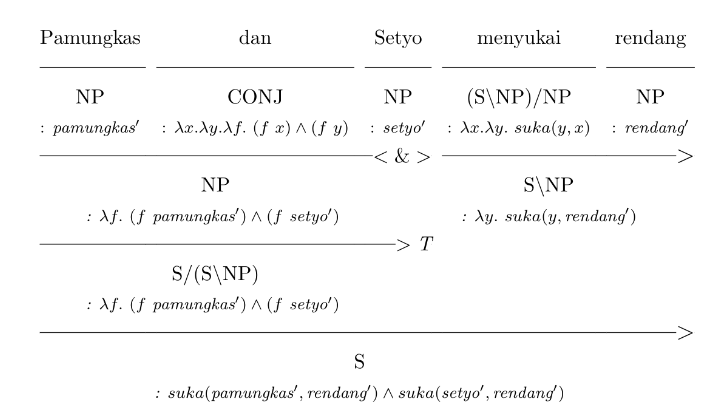
\includegraphics[width=.75\textwidth]{ccg1}
  \caption{
    Contoh CCG \textit{derivation} dengan operasi \textit{coordination},
    \textit{forward application}, dan \textit{type rising}.}
  \label{ccg-fig1}
\end{figure}

\begin{equation}\label{ccg:query:1}
  suka(\so{pamungkas}, \so{rendang}) \land suka(\so{setyo}, \so{rendang})
\end{equation}
\\


\noindent\textbf{Lambda Calculus}

\textit{Lambda calculus} ({$\lambda$}\textit{-calculus}) merupakan sebuah formalisme yang dikembangkan
oleh Alonzo Church sebagai alat yang digunakan untuk memahami konsep komputasi yang efektif
\citep{DBLP:journals/corr/Rojas15}.
Formalisme {$\lambda$}\textit{-calculus} cukup populer dan bahkan dijadikan sebagai pondasi teori bagi
paradigma pemrograman \textit{functional programming}.
Konsep utama dari {$\lambda$}\textit{-calculus} adalah apa yang disebut dengan \textit{expression}.
Suatu \textit{expression} dalam {$\lambda$}\textit{-calculus} terdiri dari tiga bagian yaitu
\textit{lambda notation} ({$\lambda$}), \textit{argument} (seperti $a$, $b$, $c$, $x$, dan lain-lain),
dan \textit{body} yang dipisahkan dengan tanda titik.
Sebagai contoh, fungsi lambda ${\lambda}x. x$ merupakan sebuah fungsi identitas yang mengambil
argumen $x$ kemudian mengembalikan nilai $x$ itu sendiri.
Dalam hal ini, terlihat bahwa notasi {$\lambda$} merupakan sebuah penanda bagi suatu fungsi lambda.
Kemudian, pengubah $x$ setelah notasi {$\lambda$} merupakan argumen dari fungsi tersebut.
Selanjutnya, tanda titik merupakan pemisah antara \textit{head} dan \textit{body} fungsi lambda.
Terakhir, setelah tanda titik adalah \textit{body} dari suatu fungsi lambda yang mana berupa
\textit{expression}.

Untuk mempermudah pemahaman, {$\lambda$}\textit{-calculus} dapat diperlakukan seperti fungsi tanpa
nama. Sebagai contoh, fungsi lambda $({\lambda}x. x + 5)$ apabila diberikan nilai $2$ sehingga
menjadi $({\lambda}x. x + 5) 2$ akan dievaluasi menjadi ${\lambda}(2). (2) + 5$.
Demikian itu, nilai yang dikembalikan oleh fungsi tersebut adalah $7$.
Sama seperti fungsi pada umumnya, konsep ini bernama \textit{substition} (substitusi).
Memahami {$\lambda$}\textit{-calculus} dirasa perlu berhubung dalam tugas akhir ini
{$\lambda$}\textit{-calculus} digunakan sebagai bentuk formal di \textit{category}
dalam konteks CCG \textit{lexicon}. Meskipun {$\lambda$}\textit{-calculus} tidak sesederhana
yang dijelaskan sebelumnya, setidaknya memahami {$\lambda$}\textit{-calculus} seperti ini
sudah cukup untuk dapat membangun \textit{supertagger} yang ada di tugas akhir ini.
\\


\noindent\textbf{CCGweb}

CCGweb\footnote{\url{https://github.com/texttheater/ccgweb}} merupakan
\textit{open source graphical annotation tool} pertama untuk CCG \citep{evang-etal-2019-ccgweb}.
Aplikasinya berbasis web dan dibangun dengan menggunakan bahasa pemrograman
Python, PHP, dan JavaScript.
Fitur yang paling menarik dari \textit{graphical annotation tool} adalah What You See Is What
You Get (WYSIWYG) yang mana berupa kemampuan untuk me-\textit{render} CCG \textit{derivation}
sesuai dengan apa yang kita lihat.
Maksudnya, CCG \textit{derivation} akan ditampilkan horizontal sesuai dengan panjang kalimatnya
kemudian hasil \textit{derivation}-nya ditampilkan vertikal seperti contoh pada
Bagian \ref{kajian-ccg}.

Untuk dapat menggunakan CCGweb, kita perlu melakukan instalasi terlebih dahulu.
Selanjutnya barulah kita dapat menambahkan kalimat-kalimat yang ingin dianotasi.
Satu instalasi CCGweb hanya dapat digunakan untuk satu proyek anotasi sehingga
apabila kita memiliki lebih dari satu proyek maka kita perlu melakukan instalasi
CCGweb yang baru.
Demikian itu, CCGtown\footnote{\url{https://github.com/wisn/ccgtown}} hadir dengan
fitur \textit{multi-project} dan tanpa perlu melakukan instalasi di komputer lokal
karena aplikasinya \textit{hosted} sehingga dapat diakses kapan pun.



\section{Sistem yang Dibangun}

CCGtown dibangun dengan menggunakan bahasa pemrograman Python dan JavaScript.
Adapun \textit{framework} yang digunakan adalah Django.
Versi awal CCGtown merupakan sebuah \textit{proof-of-concept} dari
\textit{open source graphical annotation tool} berbasis web yang dilengkapi dengan fitur
penganotasian semi-otomatis.
Bahasa pemrograman Python digunakan karena sebagian besar \textit{library} untuk CCG
sudah tersedia di PyPi \footnote{\url{https://pypi.org/}}.
Salah satu \textit{library} penting yang digunakan sebagai dasar dari fitur penganotasian
semi-otomatis adalah NTLK \footnote{\url{http://www.nltk.org/}}.
Selanjutnya, Django digunakan untuk mempercepat proses pengembangan aplikasi.
Adapun JavaScript digunakan untuk menjadikan CCGtown aplikasi berbasis web yang interaktif.

Alur kerja CCGtown pada umumnya adalah (1) pengguna melakukan registrasi, (2) pengguna
melakukan \textit{login} ke sistem, (3) pengguna membuat proyek baru, (4) pengguna
menambahkan kalimat yang ingin dianotasi, (5) pengguna melakukan anotasi kemudian melakukan
\textit{generate} CCG \textit{derivation} dan/atau melakukan modifikasi
\textit{derivation}-nya apabila diperlukan, dan (6) pengguna melakukan \textit{export}
setelah selesai melakukan anotasi. Alur kerja tersebut mempengaruhi desain sistem dari
CCGtown. Salah satunya adalah desain dari \textit{database} yang akan digunakan.
\\


\noindent\textbf{Desain Database}

CCGtown menggunakan PostgreSQL sebagai
DBMS\footnote{Database Management System}-nya.
Hal ini karena PostgreSQL memiliki kemampuan untuk menyimpan struktur data
JSON\footnote{JavaScript Object Notation} sehingga memudahkan CCGtown untuk menyimpan
format JSON dari CCG \textit{derivation} yang telah dimanipulasi oleh pengguna melalui
fitur \textit{editable CCG derivation}.
PostgreSQL juga memiliki banyak fitur lain termasuk di antaranya dukungan
dari \textit{non-relational database model} (seperti \textit{multi-model graph})
sehingga apabila di waktu yang akan datang CCGtown memerlukan perubahan signifkan
terhadap desain \textit{database}-nya tidak perlu mengganti DBMS yang digunakan.
Fitur lain seperti \textit{function} dan \textit{procedure} juga akan sangat membantu
pengembangan CCGtown di waktu yang akan datang.

CCGtown versi awal sejatinya hanya membutuhkan tiga tabel saja yaitu tabel
\textit{accounts} untuk menyimpan pengguna yang terdaftar, tabel
\textit{projects} untuk menyimpan proyek-proyek yang sudah dibuat, dan tabel
\textit{sentences} untuk menyimpan kalimat-kalimat yang akan dianotasikan.
Tiga tabel tersebut sudah cukup untuk membangun \textit{proof-of-concept} dari
alat anotasi CCG yang akan dibangun. Adapun
ERD\footnote{Entity Relationship Diagram}-nya dapat dilihat pada Gambar\ref{erd-1}.

\begin{figure}\centering\small
  \scalebox{.75}{
  \begin{tikzpicture}[node distance=1.5cm, every edge/.style={link}]
    \node[entity] (acc) {Accounts};
    \node[attribute] (acc-id) [above=of acc] {\key{ID}} edge (acc);
    \node[attribute] (acc-uuid) [above right=of acc] {\key{UUID}} edge (acc);
    \node[attribute] (acc-email) [right=of acc] {Email} edge (acc);
    \node[attribute] (acc-password) [below right=of acc] {Password} edge (acc);

    \node[relationship] (creates) [left=of acc] {Creates} edge (acc);

    \node[entity] (prj) [below=of creates] {Projects} edge (creates);
    \node[attribute] (prj-id) [above right=of prj] {\key{ID}} edge (prj);
    \node[attribute] (prj-uuid) [above left=of prj] {\key{UUID}} edge (prj);
    \node[attribute] (prj-author) [left=of prj] {Author ID} edge (prj);
    \node[attribute] (prj-name) [below left=of prj] {Name} edge (prj);
    \node[attribute] (prj-status) [below=of prj] {Status} edge (prj);
    \node[attribute] (prj-rules) [below right=of prj] {Rules} edge (prj);

    \node[relationship] (adds) [right=0.5cm and 2cm of prj] {Adds} edge (prj);

    \node[entity] (snt) [below=of adds] {Sentences} edge (adds);
    \node[attribute] (snt-id) [left=of snt] {\key{ID}} edge (snt);
    \node[attribute] (snt-uuid) [below left=of snt] {\key{UUID}} edge (snt);
    \node[attribute] (snt-project) [below=of snt] {Project ID} edge (snt);
    \node[attribute] (snt-words) [below right=of snt] {Words} edge (snt);
    \node[attribute] (snt-cats) [right=of snt] {Categories} edge (snt);
    \node[attribute] (snt-deriv) [above right=of snt] {Derivations} edge (snt);
  \end{tikzpicture}
  }
  \caption{Conceptual Entity Relationship Diagram (ERD) CCGtown}
  \label{erd-1}
\end{figure}

Masing-masing tabel memiliki dua \textit{key} yaitu $ID$ dan
$UUID$\footnote{Universally Unique IDentifier}.
$ID$ merupakan \textit{primary key} \textit{integer} dengan \textit{auto increment}
yang berfungsi sebagai \textit{identifier} untuk melakukan operasi
\textit{update} maupun \textit{delete}.
Adapun $UUID$ merupakan \textit{indexed column} yang berfungsi sebagai
\textit{indentifier} publik (dapat dilihat oleh pengguna melalui URL)
yang mana digunakan untuk operasi \textit{read}.
$ID$ tidak digunakan sebagai \textit{identifier} publik karena pengguna dapat
melakukan \textit{brute-force} untuk mencari proyek ataupun kalimat berdasarkan
$ID$ yang bukan miliknya.
Demikian itu alasan ditambahkannya atribut $UUID$.
Alasan kenapa CCGtown tetap menyimpan kolom $ID$ adalah karena $ID$ nantinya akan
digunakan untuk membuat \textit{pagination}.

Pada tabel $accounts$, selain $ID$ dan $UUID$ juga memiliki atribut $email$ dan
$password$. Masing-masing atribut tersebut menggunakan tipe data \textit{string}
atau VARCHAR di PostgreSQL.
Tabel $accounts$ memiliki hubungan \textit{one-to-many} terhadap tabel $projects$.
Adapun atribut tabel $projects$ adalah $author\_id$, $name$, $status$, dan $rules$.
Atribut $author\_id$ merupakan \textit{foreign key} (\textit{indexed}) yang
mengarah kepada tabel $accounts$ dan tipe data yang digunakan sama dengan
atribut $ID$ yang terdapat di tabel $accounts$.
Atribut $name$ menggunakan tipe data \textit{string} (VARCHAR).
Atribut $status$ menggunakan tipe data \textit{integer} yang berperan sebagai
\textit{enum} ($0$ = \textit{just created}, $1$ = \textit{in progress},
$2$ = \textit{finished}, dan $3$ = \textit{dropped}).
Tabel $projects$ memiliki hubungan \textit{one-to-many} terhadap tabel $sentences$.
Adapun atribut tabel $sentences$ adalah $project\_id$, $words$, $categories$, dan
$derivations$. Atribut $project\_id$ merupakan \textit{foreign key}
(\textit{indexed}) yang mengarah kepada tabel $projects$ dan tipe data yang digunakan
sama dengan atribut $ID$ yang terdapat di tabel $projects$.
Sisanya, atribut $words$, $categories$, dan $derivations$ menggunakan tipe data JSON.
\\


\noindent\textbf{Desain Sistem}

CCGtown sejatinya memiliki desain sistem yang cukup sederhana.
Fungsionalitas yang akan didukung untuk versi awal adalah (1) \textit{register} dan
\textit{login}, (2) manajemen proyek (CRUD\footnote{Create, Read, Update, Delete}
), (3) dan manajemen kalimat (CRUD).
Pada manajemen kalimat, CCGtown menggunakan JavaScript untuk membuat pembuatan
maupun perubahan CCG \textit{derivation} menjadi lebih interaktif.
Selain tiga fungsionalitas tersebut, CCGtown juga menambahkan fungsionalitas tambahan
seperti \textit{auto-assign category} yang dilakukan di sisi \textit{frontend}.
Kemudian, CCGtown juga menambahkan fungsionalitas tambahan di sisi \textit{backend}
yaitu CCG \textit{derivation generator} dengan memanfaatkan \textit{library} NLTK
dan kemampuan untuk melakukan \textit{export} CCG \textit{derivation} yang disimpan
di \textit{database}.

Pengguna harus terdaftar terlebih dahulu sebelum dapat melaukan anotasi sehingga
langkah awal yang harus dibangun adalah fungsionalitas \textit{register}.
Alur proses pendaftaran pengguna dapat dilihat pada Gambar \ref{flowchart:register}.
Berhubung fokus saat ini adalah \textit{proof-of-concept}, informasi yang dibutuhkan
untuk mendaftar hanyalah \textit{email} dan \textit{password}. Adapun
\textit{password confirmation} digunakan untuk memvalidasi \textit{password}
sehingga dapat mengurangi risiko pengguna melupakan
\textit{password}-nya yang baru saja di-\textit{input}.
Saat pengguna melakukan pendaftaran, sistem akan memeriksa apakah \textit{email} yang
didaftar sudah terdapat di \textit{database}.
Apabila sudah terdaftar, pengguna akan dialihkan ke halaman \textit{register} kembali
dan mendapatkan \textit{flash message} dengan keterangan "email sudah terdaftar".
Sebaliknya, sistem akan melakukan \textit{input} data tersebut ke dalam \textit{database}
lalu mengalihkan pengguna ke halaman \textit{login}.
Ketika dialihkan ke halaman \textit{login}, pengguna akan melihat \textit{flash message}
dengan keterangan "pengguna berhasil didaftarkan".
Pada tahap ini pengguna sudah dapat melakukan \textit{login} ke dalam sistem CCGtown.

\begin{figure}\centering\small
  \scalebox{.75}{
	\begin{tikzpicture}[node distance=2cm]
    \node (start) [cloud] {Start};
    \node (input) [io, below of=start, yshift=0.5cm] {\textit{Input email, password,} dan \textit{password confirmation}};
    \node (check) [process, below of=input, yshift=0.5cm] {Mencari pengguna berdasarkan \textit{email}};
    \node (is-registered) [decision, below of=check, yshift=-1.25cm] {\textit{Email} sudah terdaftar?};
    \node (registered) [process, right of=is-registered, yshift=0cm, xshift=4.5cm] {\textit{Redirect} ke halaman \textit{register}};
    \node (registering) [process, below of=is-registered, yshift=-1.75cm] {\textit{Input} informasi pengguna ke \textit{database}};
    \node (redirect) [process, below of=registering, yshift=0.5cm] {\textit{Redirect} ke halaman \textit{login}};
    \node (stop) [cloud, below of=redirect, yshift=0.5cm] {Stop};

    \draw [arrow] (start) -- (input);
    \draw [arrow] (input) -- (check);
    \draw [arrow] (check) -- (is-registered);
    \draw [arrow] (is-registered) -- node[anchor=south]{Ya} (registered);
    \draw [arrow] (registered) -- +(3,0) |- (input);
    \draw [arrow] (is-registered) -- node[anchor=east]{Tidak} (registering);
    \draw [arrow] (registering) -- (redirect);
    \draw [arrow] (redirect) -- (stop);
  \end{tikzpicture}
  }
	\caption{Alur proses pendaftaran pengguna.}
  \label{flowchart:register}
\end{figure}

Pada proses "\textit{input} informasi pengguna ke \textit{database}" CCGtown melakukan
\textit{password hashing} dengan menggunakan Bcrypt.
Informasi sensitif seperti \textit{password} sebaiknya tidak disimpan sebagai
\textit{plain text}. Demikian itu CCGtown menggunakan \textit{password hashing}.
Apabila hal buruk terjadi seperti misalnya \textit{data breach} (kebocoran data),
\textit{password} pengguna tidak dapat langsung digunakan.
Peretas perlu mencari cara untuk memecahkan \textit{password} tersebut.
Bcrypt merupakan skema \textit{password hashing} berbasis Blowfish \textit{block cipher}
yang didesain untuk lebih \textit{resistant} terhadap serangan \textit{brute-force}
\citep{bcrypt}.
Serangan \textit{brute-force} merupakan upaya peretas untuk menebak \textit{password}
dengan cara membuat \textit{wordlist} yang kemudian dicocokkan dengan \textit{hash}
yang terbentuk satu-demi-satu.
Meskipun terjadi \textit{data breach}, peretas perlu usaha ekstra untuk dapat menebak
\textit{password} dari satu pengguna.
Hal ini mengurangi kerugian yang akan dialami oleh CCGtown apabila \textit{data breach}
benar-benar terjadi.

Selanjutnya, setelah melakukan registrasi, pengguna dapat melakukan \textit{login} ke
sistem CCGtown.
Proses yang dilakukan pada umumnya sama dengan aplikasi web yang memiliki
kemampuan \textit{register} dan \textit{login}. Alur proses \textit{login} dapat dilihat
pada Gambar \ref{flowchart:login}.
Setelah pengguna melakukan \textit{input} \textit{email} dan \textit{password}-nya,
CCGtown akan melakukan pencarian di \textit{database} apakah \textit{email} yang
diberikan terdaftar. Apabila tidak terdaftar, pengguna akan dialihkan ke halaman
\textit{login} dan diberikan \textit{flash message} "\textit{Email} dan/atau
\textit{password} tidak cocok". Pesan ini diberikan agar peretas tidak dapat mencari
tahu \textit{email} mana saja yang sudah terdaftar. Selanjutnya, apabila akun
dengan \textit{email} tersebut ada, maka langkah selanjutnya adalah mencocokkan
\textit{password} yang diberikan oleh pengguna dan \textit{password} yang telah
disimpan di \textit{database}. Kemudian, sistem melakukan Bcrypt \textit{sync}.
Apabila tidak berhasil, pengguna akan dialihkan ke halaman \textit{login}
dan diberikan \textit{flash message} "\textit{Email} dan/atau \textit{password}
tidak cocok". Sebaliknya, pengguna akan dialihkan ke halaman Projects yang berisi
daftar proyek yang telah dibuat sebelumnya.

\begin{figure}\centering\small
  \scalebox{.75}{
	\begin{tikzpicture}[node distance=2cm]
    \node (start) [cloud] {Start};
    \node (input) [io, below of=start, yshift=0.5cm] {\textit{Input email} dan \textit{password}};
    \node (check) [process, below of=input, yshift=0.5cm] {Mencari pengguna berdasarkan \textit{email}};
    \node (is-registered) [decision, below of=check, yshift=-1.25cm] {\textit{Email} sudah terdaftar?};
    \node (not-registered) [process, left of=is-registered, yshift=0cm, xshift=-4.5cm] {\textit{Redirect} ke halaman \textit{login}};
    \node (logging-in) [process, below of=is-registered, yshift=-1.75cm] {Mencocokkan \textit{password} dengan Bcrypt \textit{sync}};
    \node (is-matched) [decision, below of=logging-in, yshift=-1.25cm] {\textit{Password} cocok?};
    \node (redirect) [process, below of=is-matched, yshift=-1.75cm] {\textit{Redirect} ke halaman Projects};
    \node (stop) [cloud, below of=redirect, yshift=0.5cm] {Stop};

    \draw [arrow] (start) -- (input);
    \draw [arrow] (input) -- (check);
    \draw [arrow] (check) -- (is-registered);
    \draw [arrow] (is-registered) -- node[anchor=south]{Tidak} (not-registered);
    \draw [arrow] (not-registered.north) -- +(0,0) |- (input);
    \draw [arrow] (is-registered) -- node[anchor=east]{Ya} (logging-in);
    \draw [arrow] (logging-in) -- (is-matched);
    \draw [arrow] (is-matched.west) -| +(-4.9,0) -- node[anchor=east]{Tidak} (not-registered.south);
    \draw [arrow] (is-matched) -- node[anchor=east]{Ya} (redirect);
    \draw [arrow] (redirect) -- (stop);
  \end{tikzpicture}
  }
	\caption{Alur proses \textit{login} ke sistem CCG.}
  \label{flowchart:login}
\end{figure}

Pada halaman Projects, pengguna dapat membuat proyek atau menghapus proyek.
Tidak ada fungsionalitas spesial di halaman Projects selain CRUD pada umumnya.
Satu pengguna dapat membuat banyak proyek. Tidak ada larangan tertentu terhadap penamaan
proyek. Namun, sangat disarankan memberikan nama proyek yang deskriptif seperti misalnya
"\textit{Wide-range Indonesian Dataset}". Setiap proyek memiliki status yang berbeda-beda.
Proyek yang baru saja dibuat akan memiliki status \textit{just created}.
Hal ini untuk memudahkan \textit{annotator} mencari proyek mana yang baru akan dikerjakan,
proyek mana yang sedang dikerjakan, proyek mana yang sudah selesai dikerjakan, atau
proyek mana yang tidak jadi dikerjakan. Proyek yang telah dibuat dapat disunting maupun
dihapus. Proyek yang dihapus tidak dapat dikembalikan (\textit{undo}).
Adapun penyuntingan proyek terjadi di halaman Editor.

Pada halaman Editor, pengguna dapat menyunting informasi proyek seperti nama proyek,
status proyek, dan \textit{rules} yang akan digunakan untuk melakukan \textit{generate}
CCG \textit{derivation} via NTLK. Selain itu, pengguna juga dapat menambahkan kalimat
baru yang akan dianotasi. Pengguna dapat menambahkan lebih dari satu kalimat sekaligus.
Kalimat-kalimat tersebut akan di-\textit{tokenize} menggunakan \textit{library} NLTK.
Ekstensi yang digunakan untuk proses \textit{tokenize} ini adalah punkt.
Setelah itu, barulah pengguna dapat melakukan penganotasian terhadap kalimat-kalimat yang
telah ditambahkan. Terdapat dua cara untuk memberikan anotasi yaitu secara langsung di
halaman Editor atau dapat juga dilakukan di Editable CCG Modal.
Saat ini CCGtown belum mendukung penganotasian terhadap \textit{compound words}.
CCGtown saat ini juga belum mendukung penganotasian CCG dengan semantik.
Versi awal CCGtown hanya mendukung penganotasian CCG secara sintaksis saja.

Setelah semua kata dalam suatu kalimat diberikan anotasi, pengguna dapat melakukan
\textit{generate} CCG \textit{derivation}. Hal ini dapat dilakukan berkat bantuan
\textit{library} NLTK. Kami mengambil sebuah $rules$ dari tabel $projects$ dan kemudian
kami mengambil semua $words$ serta $categories$ dari tabel $sentences$ yang merupakan
bagian dari proyek tersebut. Kolom $words$ merupakan kumpulan kata dari kalimat yang telah
di-\textit{tokenize}. Adapun kolom $categories$ merupakan anotasi CCG \textit{category}-nya.
\textit{Pseudocode} untuk \textit{generate} CCG \textit{derivation} dapat dilihat pada
Kode \ref{code:ccg-gen} dengan asumsi anotasi yang diberikan absah (dapat dibuat CCG
\textit{derivation}-nya). Kode $next$ tersebut akan mengambil satu dari banyak
kemungkinan \textit{derivation} yang dapat dibuat. Contoh \textit{object} yang
di-\textit{return} dapat dilihat pada Kode \ref{code:ccg-gen-example}.
Untuk kepentingan \textit{rendering} di sisi \textit{frontend}, \textit{key} seperti
$from$ dan $to$ sangat diperlukan. \textit{Key} $from$ dan \textit{key} $to$
merepresentasikan \textit{index} posisi terhadap \textit{array} $words$.
Dengan bantuan kedua \textit{key} tersebut, \textit{frontend} dapat melakukan kalkulasi
posisi masing-masing elemen yang terdapat di \textit{object} $derivations$.

\begin{lstlisting}[
  language=python,
  firstnumber=1,
  caption={Pseudocode untuk melakukan \textit{generate} CCG \textit{derivation}.},
  label={code:ccg-gen}
]
from nltk.ccg import chart, lexicon

def generateCCGDerivation(rules, words, categories, target_words):
    lex = rules + '\n\n'
    for i in range(len(words)):
        lex += words[i] + ' => ' + categories[i] + '\n'

    lex = lexicon.parseLexicon(lex)
    parser = chart.CCGChartParser(lex, chart.DefaultRuleSet)
    result = next(parser.parse(target_words))
    derivations = makeCCGDeriv(result)

    return derivations
\end{lstlisting}

Kode \ref{code:ccg-gen-example} didapatkan dari fungsi $makeCCGDeriv$ yang terdapat pada
Kode \ref{code:ccg-gen}. Fungsi $makeCCGDeriv$ sederhananya mengambil $Tree$ yang didapatkan
dari $parser.parse$ kemudian melakukan \textit{tree traversal}. Semua \textit{leaf}, diambil
dari paling "kiri", diletakkan di elemen pertama $derivations$. Selanjutnya, kita berjalan
melalui \textit{parent} dari \textit{leaf} tersebut hingga ke \textit{root} mencari bentuk CCG
\textit{derivation}-nya. Banyaknya baris yang dibutuhkan oleh CCG \textit{derivation} dapat
dilihat dari \textit{height} yang dimiliki oleh $Tree$ tersebut. Kemudian, hasil dari CCG
\textit{derivation} (umumnya berupa $S$) merupakan elemen terakhir $derivations$.
Adapun hasil \textit{render} di sisi \textit{frontend}-nya dapat dilihat pada Gambar
\ref{ui:deriv-generated}.

\begin{lstlisting}[
  language=json,
  firstnumber=1,
  caption={Contoh \textit{derivations object} yang di-\textit{return}.},
  label={code:ccg-gen-example}
]
[
  [
    { "to": 0, "from": 0, "word": "You" },
    { "to": 1, "from": 1, "word": "prefer" },
    { "to": 2, "from": 2, "word": "that" },
    { "to": 3, "from": 3, "word": "cake" }
  ],
  [
    { "to": 0, "from": 0, "category": "NP" },
    { "to": 1, "from": 1, "category": "((S\NP)/NP)" },
    { "to": 2, "from": 2, "category": "(NP/N)" },
    { "to": 3, "from": 3, "category": "N" }
  ],
  [
    { "to": 3, "from": 2, "category": "NP", "operator": ">" }
  ],
  [
    { "to": 3, "from": 1, "category": "(S\NP)", "operator": ">" }
  ],
  [
    { "to": 3, "from": 0, "category": "S", "operator": "<" }
  ]
]
\end{lstlisting}

Selain memiliki kemampuan untuk melakukan \textit{generate} CCG \textit{derivation},
CCGtown juga memiliki kemampuan untuk melakukan \textit{auto-assign} CCG \textit{category}.
Token kata yang sudah dianotasi oleh pengguna akan disimpan ke dalam suatu \textit{dictionary}.
Untuk setiap kata yang belum dianotasi, CCGtown akan memeriksa apakah token kata tersebut
sebelumnya sudah dianotasi. Apabila sudah, CCGtown akan memberikan anotasi secara otomatis.
Suatu token kata mungkin memiliki lebih dari satu anotasi. CCGtown hanya akan mengambil satu
anotasi saja. Akibatnya, pengguna sebaiknya tetap melakukan peninjauan.
Kendati demikian, setidaknya kegiatan anotasi yang repetitif dapat berkurang sehingga memudahkan
dan mempercepat proses anotasi.
\\


\noindent\textbf{Pertimbangan UI/UX}

Secara keseluruhan, CCGtown memiliki halaman rumah (\textit{homepage}), halaman \textit{register},
halaman \textit{login}, halaman Projects, dan halaman Editor.
Halaman \textit{register} dan halaman \textit{login} pada dasarnya sama.
Perbedaannya hanya terdapat di jumlah \textit{field} yang diminta serta \textit{copy writting}
yang sedikit berbeda. Desain UI\footnote{User Interface} serta UX\footnote{User Experience}
CCGtown dibuat dengan fokus untuk mempermudah penggunaan \textit{annotation tool} ini.
CCGtown tidak menggunakan banyak warna. Hal ini untuk mengurangi kelelahan pada mata pengguna.
CCGtown menggunakan bahasa Inggris di antarmukanya karena target pengguna CCGtown adalah
pengguna baik dari Indonesia yang mengerti bahasa Inggris maupun pengguna dari manca negara.

CCGtown menggunakan UIKit\footnote{\url{https://getuikit.com/}} sebagai \textit{framework}
untuk melakukan implementasi desain web-nya. UIKit dipilih karena komponen-komponen yang
dibutuhkan CCGtown sudah tersedia sehingga CCGtown hanya perlu melakukan sedikit penyesuaian
seperti penambahan warna, pengaturan jarak (\textit{margin} dan \textit{padding}), dan sejenisnya.
UIKit juga sudah menyediakan kumpulan \textit{icons} yang dapat langsung digunakan.
Hal ini mengakibatkan proses pengembangan desain web CCGtown dapat diselesaikan dalam waktu yang
relatif cukup singkat.

Warna utama (\textit{primary color}) CCGtown adalah warna ungu.
Berdasarkan psikologi warna, warna ungu adalah warna fantasi dan magis.
CCGtown dapat men-\textit{generate} CCG \textit{derivation} dan melakukan \textit{auto-assign}
CCG \textit{category} sehingga memiliki sifat yang seakan-akan mengandung magi (sihir).
Selain itu, ungu menumbuhkan kreativitas dengan membangkitkan indra kita sambil mempromosikan
ketenangan yang diperlukan untuk melakukan pengamatan yang intuitif dan berwawasan.
Warna ungu banyak digunakan oleh \textit{homepage} seperti yang terlihat pada Gambar
\ref{ui:homepage}. Halaman rumah CCGtown didesain sederhana dan langsung kepada intinya.
Halaman rumah CCGtown menampilkan beberapa fitur yang dapat menjadi alasan bagi pengguna
untuk menggunakan CCGtown. Selain itu, halaman rumah CCGtown juga menampilkan demonstrasi
singkat dengan gambar animasi proses penganotasian di CCGtown. Demonstrasi singkat
diberikan untuk memberikan gambaran kepada calon pengguna tentang betapa mudahnya
menggunakan CCGtown untuk menganotasi CCG.

Pada Gambar \ref{ui:register} dan Gambar \ref{ui:login}, terlihat bahwasannya halaman
\textit{register} dan halaman \textit{login} pada dasarnya sama. Pada halaman
\textit{register}, informasi yang dibutuhkan hanyalah \textit{email address} dan
\textit{password} (dengan tambahan \textit{password confirmation} untuk validasi).
Hal ini agar pengguna dapat dengan mudah mendaftar tanpa perlu mengisi banyak \textit{field}
terlebih dahulu sebelum dapat menggunakan CCGtown. Selain itu, informasi lain dari
pengguna saat ini belum dibutuhkan. Apabila terjadi perubahan mengenai data pengguna,
pengguna dapat memperbarui datanya di kemudian hari melaui halaman lain seperti halaman profil
yang mungkin saja akan ditambahkan di CCGtown versi berikutnya.

CCGtown menggunakan \textit{flash message} berupa \textit{toast} untuk setiap pesan
\textit{feedback} yang diberikan oleh sisi \textit{backend}. Sebagai contoh, pada Gambar
\ref{ui:flash-message} di bagian pojok kanan bawah merupakan pesan \textit{feedback}
yang memberikan informasi bahwasannya kombinasi \textit{email} dan/atau \textit{password}
tidak cocok sehingga pengguna tidak dapat \textit{login}. Notifikasi \textit{toast} tersebut
dapat langsung ditutup oleh pengguna atau akan hilang dengan sendirinya dalam waktu sekitar
lima detik. Penggunaan \textit{toast} yang muncul dari bawah dengan warna ungu tersebut
dapat mengalihkan perhatian pengguna sehingga pengguna menyadari pesan yang disampaikan oleh
\textit{backend} CCGtown.

Selanjutnya, dengan asumsi pengguna baru saja mendaftar kemudian melakukan \textit{login},
pengguna akan dialihkan ke halaman Projects. Halaman Projects tersebut berada di dalam
\textit{empty state} karena pengguna belum membuat satupun proyek. Seperti yang dapat
dilihat pada Gambar \ref{ui:projects-empty}, pengguna dapat melihat instruksi apa yang
harus ia lakukan yang mana dalam hal ini adalah membuat proyek baru.
Sebaliknya, apabila pengguna telah membuat proyek maka tampilan yang dilihat akan
seperti pada Gambar \ref{ui:projects}. Pengguna dapat membuka halaman Editor dengan
cara melakukan klik di nama proyek maupun di ikon \textit{edit}. Selain itu,
pengguna juga dapat langsung melakukan \textit{export to JSON} melakukan klik di ikon
\textit{download}. Apabila pengguna merasa tidak lagi memerlukan suatu proyek, maka
pengguna dapat menghapusnya dengan melakukan klik di ikon \textit{trash}.

Setelah membuat proyek baru, pengguna akan melihat halaman Editor dalam
\textit{empty state} seperti yang dapat dilihat pada Gambar \ref{ui:editor-empty}.
Pada bagian kanan halaman Editor, terdapat beberapa \textit{section} yaitu
Project Detail yang dapat digunakan untuk mengubah nama proyek dan status proyek,
Automation Rules yang akan digunakan oleh NLTK untuk melakukan \textit{generate}
CCG \textit{derivation}, serta CCG Lexicons yang menampilkan statistik dari jenis
sintaksis CCG yang telah dianotasikan dan berapa kali ia dianotasikan.
Untuk dapat menambahkan kalimat baru, pengguna hanya perlu melakukan klik di
tombol "Add Sentences". Setelah itu, pengguna dapat langsung melakukan penganotasian
seperti yang terlihat pada Gambar \ref{ui:editor-annotating}. Apabila pengguna telah
memberikan anotasi ke semua token kata yang ada di kalimat tersebut, pengguna dapat
melakukan \textit{generate} CCG \textit{derivation}. Hasil dari \textit{generate} CCG
\textit{derivation} tersebut dapat dilihat pada Gambar \ref{ui:deriv-generated}.

Pengguna juga dapat langsung mengubah CCG \textit{derivation} suatu kalimat secara
langsung. Contohnya dapat dilihat pada Gambar \ref{ui:deriv-progress}.
Pengguna dapat memberikan anotasi ke token kata di \textit{modal} (\textit{editable}
CCG \textit{derivation}) tersebut. Pengguna dapat menambahkan beberapa baris kosong
sekaligus yang kemudian akan diisi oleh CCG \textit{derivation} dari kalimat tersebut.
Warna abu-abu menunjukkan bahwa konfigurasi dari CCG \textit{derivation} di baris tersebut
masih kosong. Kemudian, warna ungu menunjukkan bahwa pada bagian tersebut (baik anotasi
maupun operator) tidak diisi. Perbedaan ini diberikan untuk memberikan pengguna
\textit{awareness} mengenai mana saja bagian yang harus diisi atau dilengkapi.
Adapun konfigurasi \textit{derivation}-nya terlihat pada Gambar \ref{ui:deriv-configure}.
Dengan kemampuan ini pengguna dapat melakukan \textit{generate} kemudian apabila ada
\textit{derivation} yang dirasa kurang cocok maka pengguna dapat langsung melakukan
perubahan dengan mudah dan interaktif.



\section{Evaluasi}

TBA.
% Bagian ini berisi dua sub-bagian, yaitu Hasil Pengujian dan Analisis Hasil Pengujian. Pengujian dan analisis yang dilakukan selaras dengan tujuan TA sebagaimana dinyatakan dalam Pendahuluan.

\subsection{Hasil Pengujian}

TBA.
% Pertama, tampilkan hasil pengujian yang paling utama. Kemudian hasil-hasil yang lebih detil ditampilkan setelah hasil yang utama. Mengingat tinggi atau rendah, baik atau jeleknya hasil pengujian bersifat relatif, maka sangat dianjurkan ada pembanding (baseline) yang membandingkan dengan algoritma atau pendekatan yang dipilih untuk TA. Pembanding dijalankan pada lingkungan (termasuk data set) yang sama.

% Pilih tabel atau jenis diagram yang sesuai untuk menampilkan hasil pengujian. 


\subsection{Analisis Hasil Pengujian}

TBA.
%  Analisis merupakan salah satu bagian yang penting untuk TA. Pada TA S1 tidak dituntut untuk mendapatkan hasil performasi yang lebih bagus dibandingkan dengan baseline yang populer, yang dituntut adalah membuat analisis yang lengkap. Menganalisis pengaruh kondisi-kondisi yang berbeda (seperti parameter, jenis data, threshold, dan sub-sistem) yang digunakan. 
 
%  Cara sitasi adalah sebagai berikut: \citep{van2002fundamentals} untuk buku, \citep{ochoa2003hybrid} untuk \textit{paper}, dan \citep{Budi} untuk website.
   
   
\section{Kesimpulan}

TBA.
%  \noindent Bagian Kesimpulan memuat kesimpulan dan Saran (\textit{Future Work}), bisa dituliskan dalam poin-poin ataupun paragraf-paragraf. Semua poin kesimpulan diambil dari hasil pengujian dan analisis hasil pengujian sehingga tidak ada kesimpulan dari teori ataupun nalar semata. Sebagaimana sudah disebutkan pada bagian sebelumnya, pengujian dan analisis harus sesuai dengan tujuan TA. Jadi kesimpulan-kesimpulan yang dituliskan selaras dengan seluruh tujuan TA. 
 


\bibliographystyle{abbrv}
\bibliography{references}

\section*{Lampiran}

\begin{figure}[b]\centering
  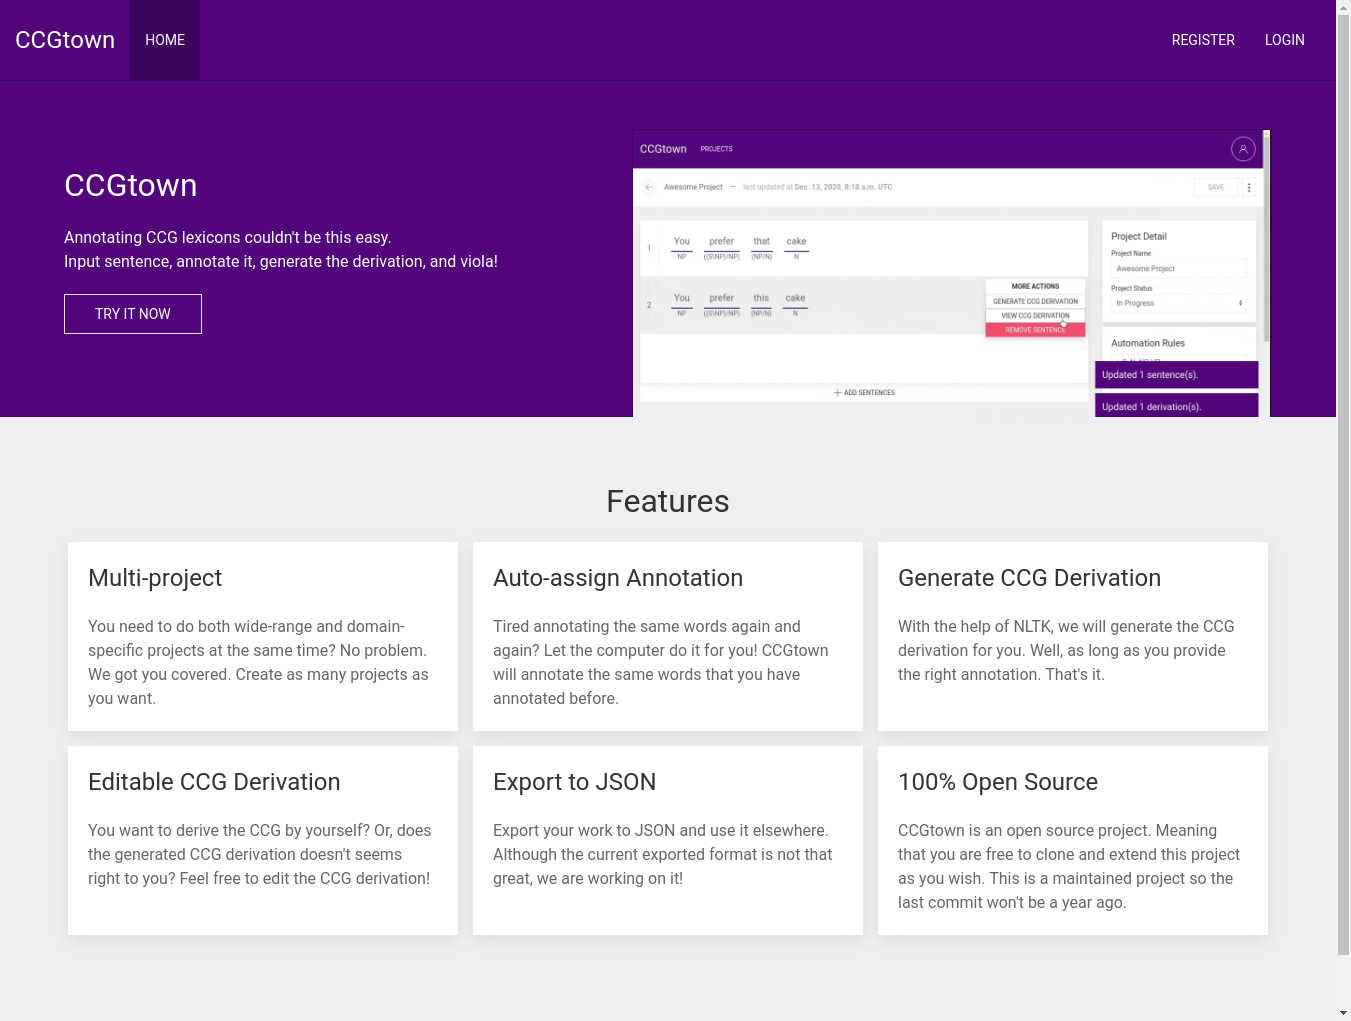
\includegraphics[width=\textwidth]{homepage}
  \caption{Antarmuka \textit{homepage} CCGtown.}
  \label{ui:homepage}
\end{figure}

\begin{figure}\centering
  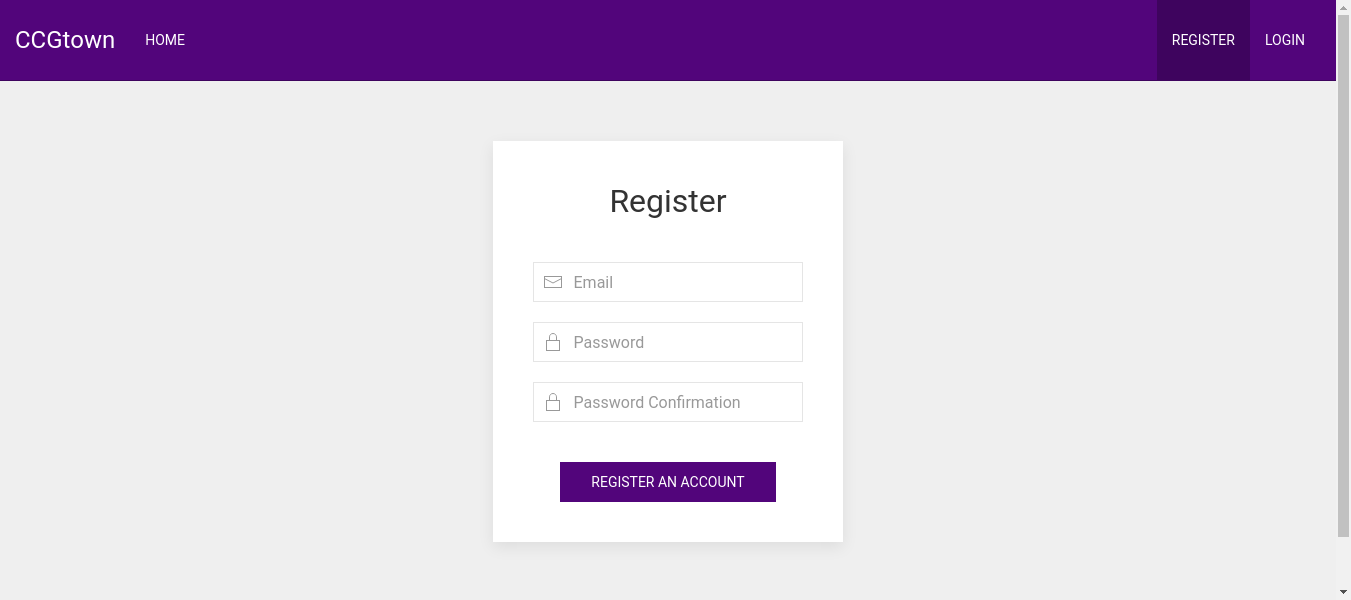
\includegraphics[width=\textwidth]{register}
  \caption{Antarmuka halaman \textit{register} CCGtown.}
  \label{ui:register}
\end{figure}

\begin{figure}\centering
  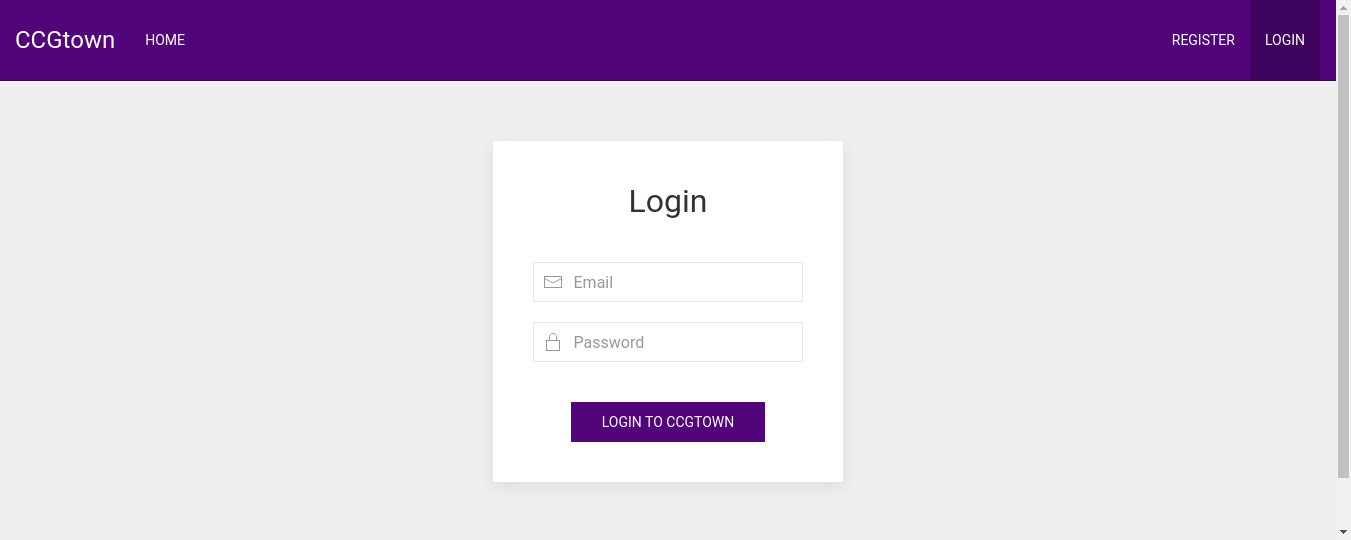
\includegraphics[width=\textwidth]{login}
  \caption{Antarmuka halaman \textit{login} CCGtown.}
  \label{ui:login}
\end{figure}

\begin{figure}\centering
  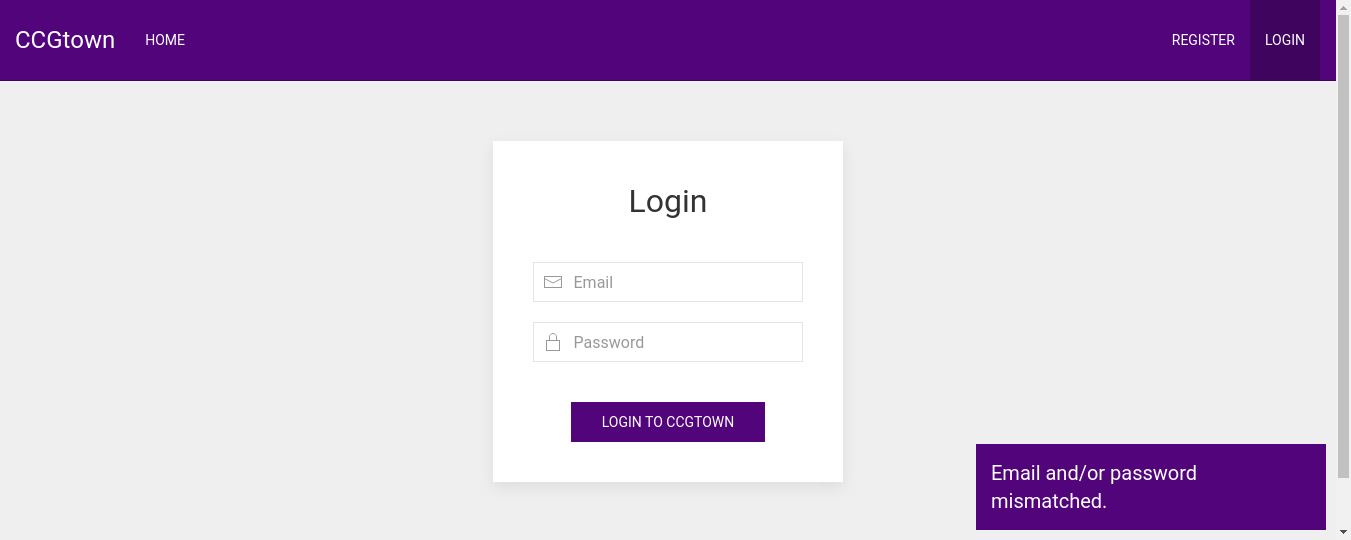
\includegraphics[width=\textwidth]{flash-message}
  \caption{Antarmuka halaman \textit{login} CCGtown dengan \textit{toast}.}
  \label{ui:flash-message}
\end{figure}

\begin{figure}\centering
  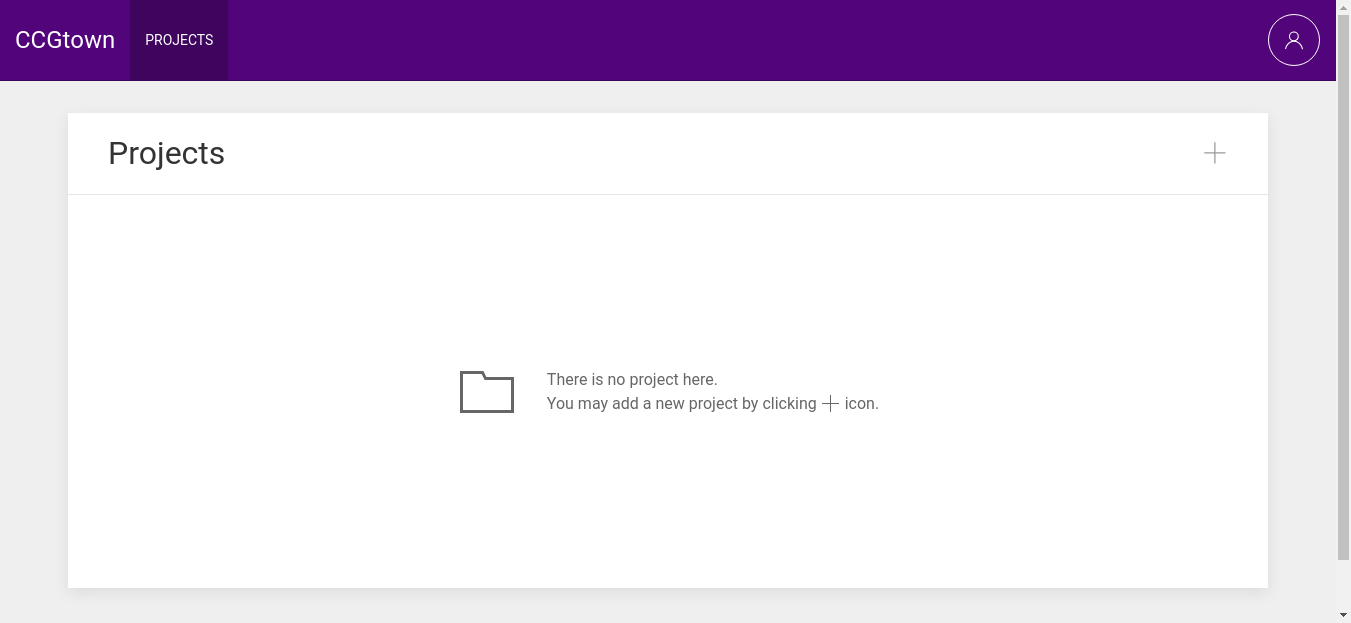
\includegraphics[width=\textwidth]{projects-empty}
  \caption{Antarmuka halaman Projects saat dalam \textit{empty state}.}
  \label{ui:projects-empty}
\end{figure}

\begin{figure}\centering
  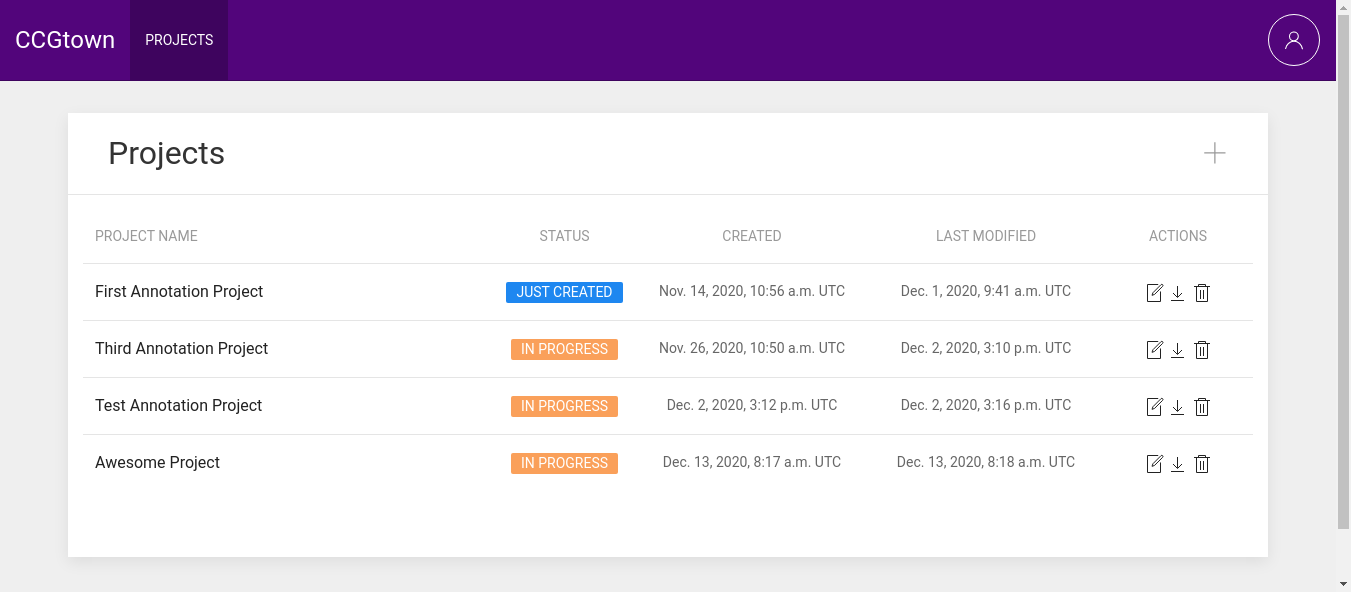
\includegraphics[width=\textwidth]{projects}
  \caption{Antarmuka halaman Projects CCGtown.}
  \label{ui:projects}
\end{figure}

\begin{figure}\centering
  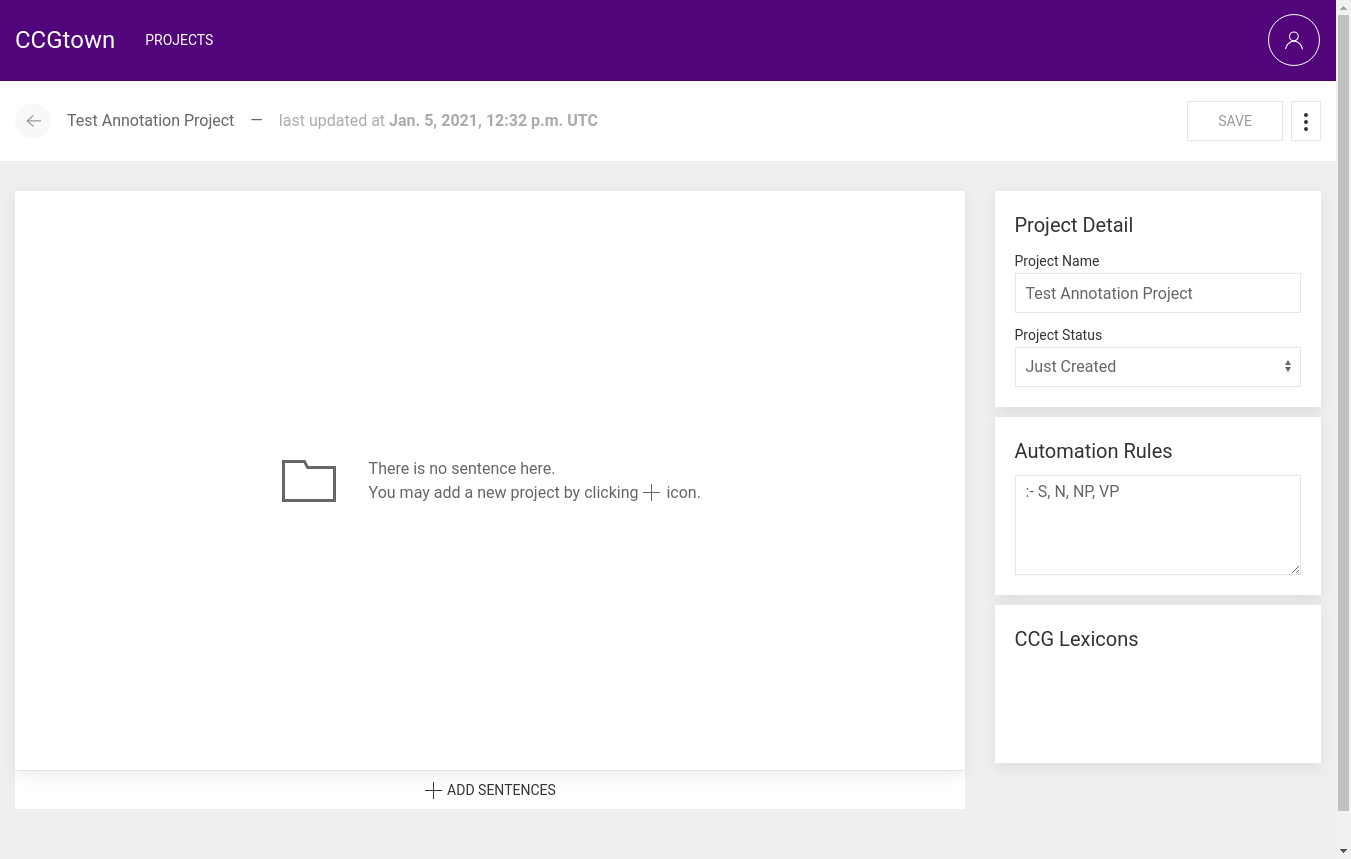
\includegraphics[width=\textwidth]{editor-empty}
  \caption{Antarmuka halaman Editor saat dalam \textit{empty state}.}
  \label{ui:editor-empty}
\end{figure}

\begin{figure}\centering
  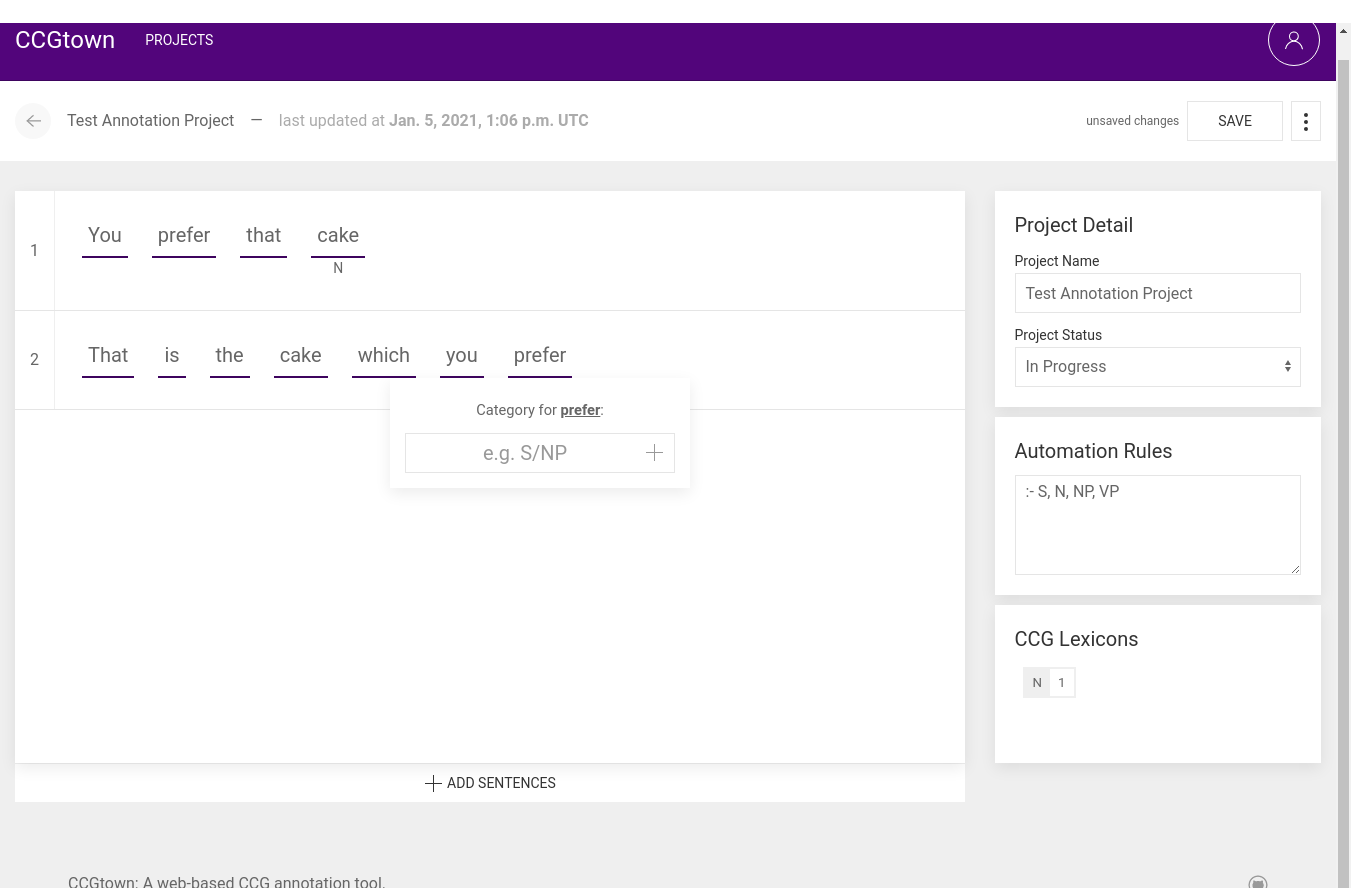
\includegraphics[width=\textwidth]{editor-annotating}
  \caption{Antarmuka halaman Editor saat melakukan penganotasian.}
  \label{ui:editor-annotating}
\end{figure}

\begin{figure}\centering
  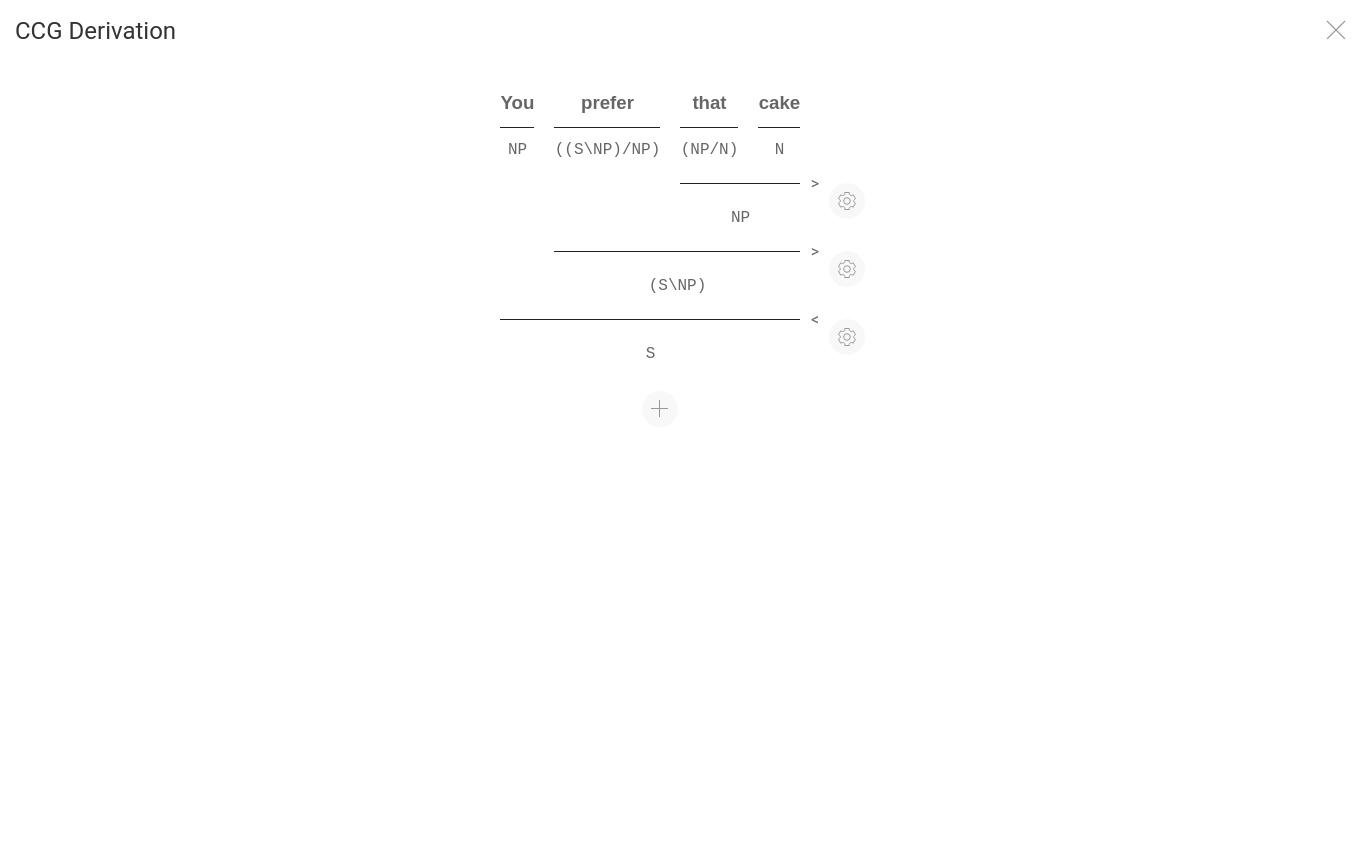
\includegraphics[width=\textwidth]{ccg-derv-generated}
  \caption{Antarmuka CCG \textit{derivation} yang telah di-\textit{generate}.}
  \label{ui:deriv-generated}
\end{figure}

\begin{figure}\centering
  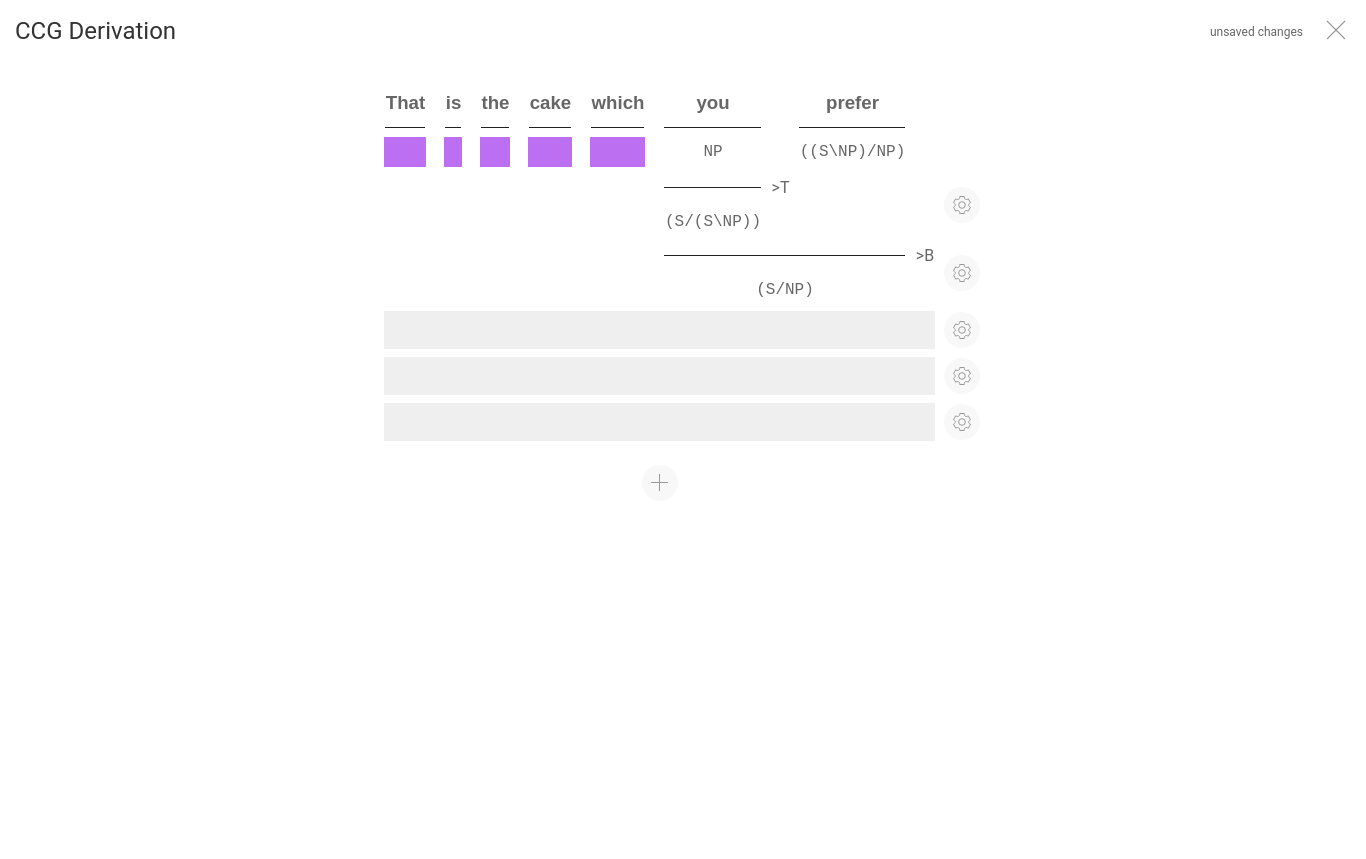
\includegraphics[width=\textwidth]{ccg-derv-progress}
  \caption{Antarmuka \textit{editable} CCG \textit{derivation} CCGtown.}
  \label{ui:deriv-progress}
\end{figure}

\begin{figure}\centering
  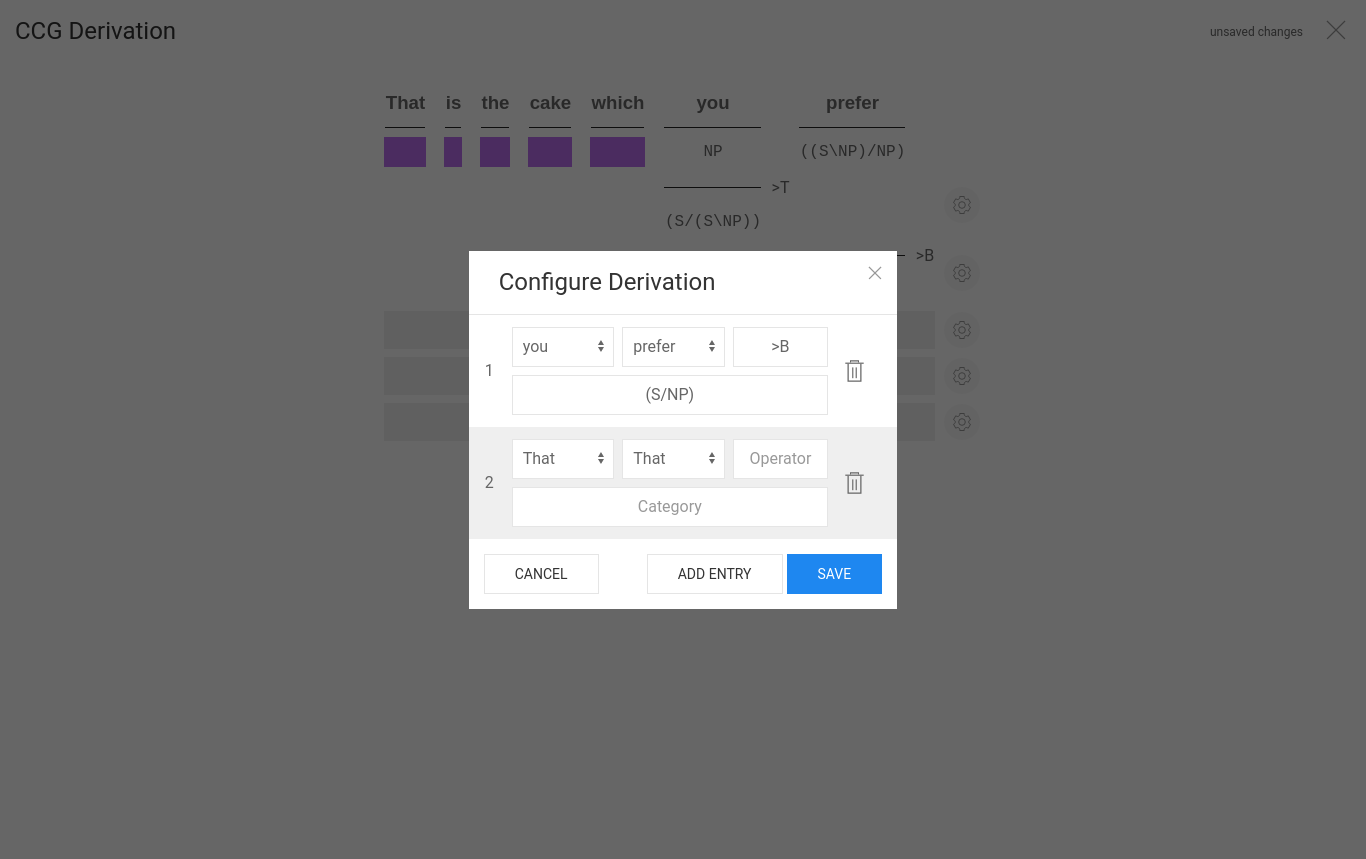
\includegraphics[width=\textwidth]{ccg-derv-configure}
  \caption{Antarmuka konfigurasi dari \textit{editable} CCG \textit{derivation} CCGtown.}
  \label{ui:deriv-configure}
\end{figure}
